% !TeX root = ../main.tex
\chapter{Implementation}
\label{ch:implementation}

This chapter presents key implementation mechanisms of the HPC Sorting Serious Game. It covers the core game logic, multiplayer synchronization protocol, barrier synchronization (a direct pedagogical mapping to \texttt{\#pragma omp barrier}), the web-export compatibility patch, and development observability tooling. Tool/framework selection rationale is documented in Chapter~\ref{ch:methodology}, architectural decisions in Chapter~\ref{ch:architecture}, and effectiveness evaluation in Chapter~\ref{ch:results}.

The complete source code is available in the project repository \citep{github_project}. External tool and framework links are listed in Appendix~\ref{app:d:tool-links}.

%-----------------------------------------------------------------------
\section{Implementation Focus Areas}
\label{sec:impl-core-components}

The implementation evidence is organized around six high-impact concerns:
\begin{itemize}
    \item card management and sorting correctness,
    \item component reuse through inheritance (\texttt{CardManager} $\to$ \texttt{MultiplayerCardManager}),
    \item network state serialization and synchronization protocol,
    \item barrier synchronization as a pedagogical feature,
    \item web-export compatibility patching,
    \item observability and debuggability for multiplayer faults.
\end{itemize}

%-----------------------------------------------------------------------
\section{Card Management and Sorting Correctness}
\label{sec:singleplayer-implementation}

The single-player card management logic resides in \texttt{card\_manager.gd} (705~lines), which serves as both the standalone game controller and the base class for multiplayer extension.

%-----------------------------------------------------------------------
\subsection{Card Generation and Initialization}
\label{subsec:card-generation}

Card generation supports configurable counts (10--200) with optional unique or repeated values. The initialization sequence in \texttt{\_ready()} follows a deterministic pipeline:

\begin{lstlisting}[caption={Card manager initialization pipeline (card\_manager.gd)}]
func _ready():
    if num_cards < 1:
        num_cards = 1
    values = generate_random_values()
    sorted_all = values.duplicate()
    sorted_all.sort()

    adjust_container_spacing()
    cards_array = generate_completed_card_array(values)
    sorted_cards_array = generate_completed_card_array(sorted_all, "SortedCard_")
    fill_card_container(cards_array, card_container)
    fill_card_container(sorted_cards_array, sorted_cards_container)
    slots = create_buffer_slots()
    _connect_signals()
\end{lstlisting}

Each card is instantiated from a preloaded scene, assigned a numeric value and a color derived from the value (for visual distinctiveness), and placed in a scrollable \texttt{HBoxContainer}. A parallel sorted reference array is generated so players can optionally view the target ordering.

%-----------------------------------------------------------------------
\subsection{Sorting Validation}
\label{subsec:sorting-validation}

Sorting validation is the completion contract used in both single-player and multiplayer modes. The actual implementation iterates over the card container's children (the authoritative UI ordering):

\begin{lstlisting}[caption={Sorting validation (card\_manager.gd, line 645)}]
func check_sorting_order() -> bool:
    var sorted_correctly = true
    if card_container.get_child_count() != num_cards:
        return false
    var cards_in_container: Array[Card] = []
    for child in card_container.get_children():
        if child is Card:
            cards_in_container.append(child as Card)
    for i in range(1, cards_in_container.size()):
        var current_card = cards_in_container[i].value
        var previous_card = cards_in_container[i - 1].value
        if current_card < previous_card:
            sorted_correctly = false
            break
    return sorted_correctly
\end{lstlisting}

This mechanism provides a deterministic completion criterion independent of UI animation state and network timing. Notably, validation checks the \emph{scene tree child order} rather than an abstract array, ensuring that what the player sees matches what is validated (see Chapter~\ref{ch:results}, Section~\ref{sec:requirements-comparison}).

%-----------------------------------------------------------------------
\subsection{Buffer Contiguity Check}
\label{subsec:buffer-contiguity}

Players use private buffer zones (simulating thread-local storage) to temporarily hold cards during sorting. A buffer contiguity check validates that cards in the buffer form a contiguous subsequence of the sorted target:

\begin{lstlisting}[caption={Buffer contiguity validation (card\_manager.gd, line 693)}]
func check_player_buffer_contiguity() -> bool:
    var buffer_values = []
    for slot in slots:
        if slot.occupied_by == null:
            return false
        buffer_values.append(slot.occupied_by.value)
    return SubarrayUtils.is_contiguous_subarray(sorted_all, buffer_values)
\end{lstlisting}

This constraint reinforces the pedagogical mapping: just as a thread in an OpenMP program should work on a logically coherent subset of data, players must select contiguous card ranges for their buffers.

%-----------------------------------------------------------------------
\section{Component Reuse: CardManager Inheritance}
\label{sec:component-reuse}

The multiplayer game controller, \texttt{MultiplayerCardManager} (1143~lines), explicitly extends the single-player \texttt{CardManager}:

\begin{lstlisting}[caption={Multiplayer extension declaration (multiplayer\_card\_manager.gd, line 1)}]
extends "res://scenes/CardScene/scripts/card_manager.gd"
class_name MultiplayerCardManager
\end{lstlisting}

This inheritance structure allows the multiplayer mode to reuse all card generation, UI layout, sorting validation, and buffer management logic while adding:
\begin{itemize}
    \item host/client role differentiation,
    \item network state serialization (via \texttt{CardState}),
    \item GDSync function exposure for remote procedure calls,
    \item barrier synchronization integration.
\end{itemize}

The multiplayer \texttt{\_ready()} overrides the parent to branch on host vs.\ client role:

\begin{lstlisting}[caption={Multiplayer initialization with host/client branching (multiplayer\_card\_manager.gd)}]
func _ready():
    is_host = ConnectionManager.am_i_host()
    my_client_id = ConnectionManager.get_my_client_id()

    barrier_manager = BarrierManager.new()
    barrier_manager.set_barrier_mode(Settings.barrier_mode)
    barrier_manager.barrier_state_changed.connect(_on_barrier_state_changed)

    setup_multiplayer_sync()

    if is_host:
        super._ready()
        await get_tree().process_frame
        broadcast_initial_game_state()
        game_state_synced = true
    else:
        _initialize_client_structure()
        await get_tree().create_timer(0.5).timeout
        request_game_state_from_host()
\end{lstlisting}

The host executes the parent \texttt{\_ready()} (generating cards normally) and then broadcasts the initial state. Clients initialize an empty UI structure and request the authoritative game state from the host, avoiding duplicate card generation that would cause divergence.

%-----------------------------------------------------------------------
\section{Multiplayer Synchronization Protocol}
\label{sec:multiplayer-implementation}

%-----------------------------------------------------------------------
\subsection{CardState Serialization}
\label{subsec:cardstate-serialization}

All card state transmitted over the network is serialized through a dedicated \texttt{CardState} inner class:

\begin{lstlisting}[caption={CardState transport protocol (multiplayer\_card\_manager.gd, lines 6--49)}]
class CardState:
    var value: int
    var index: int
    var original_index: int
    var in_container: bool
    var in_buffer: bool
    var buffer_owner: int

    func to_dict() -> Dictionary:
        return {
            "value": value,
            "index": index,
            "original_index": original_index,
            "in_container": in_container,
            "in_buffer": in_buffer,
            "buffer_owner": buffer_owner
        }

    static func from_dict(data: Dictionary) -> CardState:
        return CardState.new(
            data.get("value", 0),
            data.get("index", -1),
            data.get("original_index", -1),
            data.get("in_container", true),
            data.get("in_buffer", false),
            data.get("buffer_owner", -1)
        )
\end{lstlisting}

\texttt{CardState} captures whether a card is in the shared container or in a player's private buffer, and who owns it. This explicit serialization boundary ensures that network payloads are minimal and self-describing, and that deserialization on the receiving client produces a deterministic scene state.

%-----------------------------------------------------------------------
\subsection{Lobby and Session Lifecycle}
\label{subsec:lobby-system}

The lobby manages session creation/joining and readiness transitions before gameplay authority is established.

\begin{enumerate}
    \item Player creates room or enters room code
    \item Connection to signaling server via HTTP/SSE
    \item Peer handshake with host
    \item Players appear in lobby list
    \item Host configures game settings (card count, buffer size, barrier mode)
    \item Host starts game, triggering scene transition to multiplayer gameplay
\end{enumerate}

\begin{figure}[htbp]
    \centering
    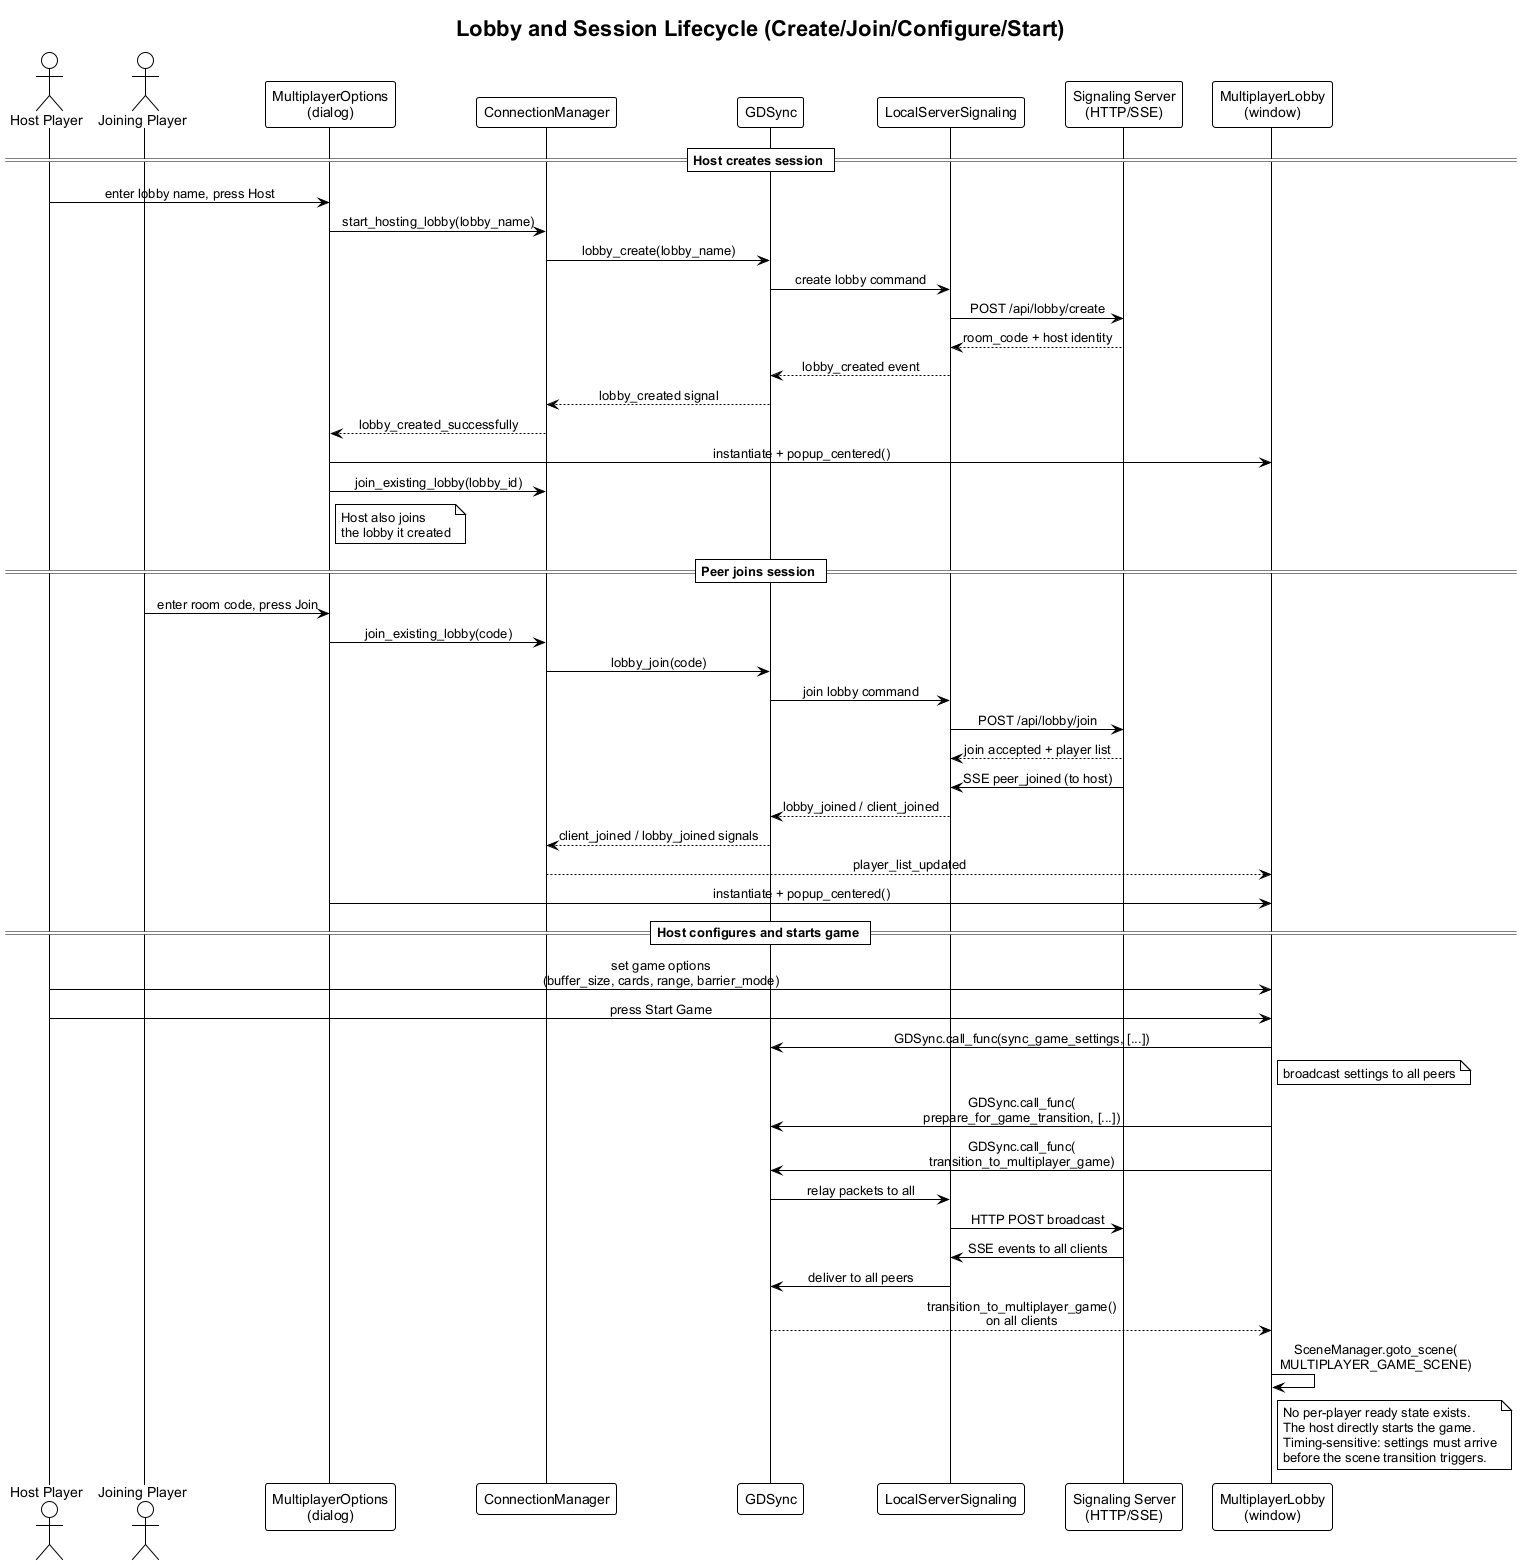
\includegraphics[width=0.92\textwidth]{figures/diagrams/lobby-session-lifecycle-sequence}
    \caption{Lobby and session lifecycle from room creation/join to synchronized game start}
    \label{fig:lobby-session-lifecycle-sequence}
\end{figure}

%-----------------------------------------------------------------------
\subsection{GDSync Function Exposure}
\label{subsec:impl-gdsync-integration}

GDSync provides high-level networking abstractions. For this thesis, the project uses an author-maintained GDSync fork that includes a fix required for the web-export workflow \citep{gdsync_fork}. A pull request with this fix was submitted upstream \citep{gdsync_framework}.

Rather than using decorator-based annotations, the actual GDSync integration uses explicit function exposure. The \texttt{setup\_multiplayer\_sync()} method registers all remotely callable functions:

\begin{lstlisting}[caption={GDSync function exposure (multiplayer\_card\_manager.gd)}]
func setup_multiplayer_sync():
    GDSync.expose_func(self.sync_complete_game_state)
    GDSync.expose_func(self.sync_card_moved)
    GDSync.expose_func(self.sync_card_entered_buffer)
    GDSync.expose_func(self.sync_card_left_buffer)
    GDSync.expose_func(self.sync_timer_state)
    GDSync.expose_func(self.sync_game_finished)
    GDSync.expose_func(self.send_current_state_to)
    # Barrier synchronization functions
    GDSync.expose_func(self.barrier_thread_reached)
    GDSync.expose_func(self.barrier_activate)
    GDSync.expose_func(self.barrier_card_picked)
    GDSync.expose_func(self.barrier_release)
\end{lstlisting}

Remote calls are then dispatched via \texttt{GDSync.call\_func()} (broadcast) or \texttt{GDSync.call\_func\_on()} (targeted to a specific peer). This explicit exposure model was required because GDSync's ``protected mode'' silently drops calls to unexposed functions (see Chapter~\ref{ch:problems}, Section~\ref{subsec:protected-mode-issue}).

%-----------------------------------------------------------------------
\subsection{State Broadcast and Reconciliation}
\label{subsec:state-broadcast}

When a card is placed in the main container (shared memory), the multiplayer manager overrides the parent handler to broadcast the move:

\begin{lstlisting}[caption={Card movement broadcast (multiplayer\_card\_manager.gd)}]
func _on_card_placed_in_container(
    dropped_card: Card = null,
    was_in_buffer: bool = false,
    original_slot: Variant = null
):
    super._on_card_placed_in_container()
    await get_tree().process_frame
    var new_index = moved_card.get_index()

    if was_in_buffer:
        GDSync.call_func(
            self.sync_card_left_buffer,
            [moved_card.value, my_client_id, new_index]
        )
    else:
        GDSync.call_func(
            self.sync_card_moved,
            [moved_card.value, moved_card.original_index,
             new_index, my_client_id]
        )
\end{lstlisting}

Clients receiving a \texttt{sync\_card\_moved} call skip the update if it originated from themselves (preventing echo loops), then reposition the card in their local scene tree:

\begin{lstlisting}[caption={Remote card movement handler (multiplayer\_card\_manager.gd)}]
func sync_card_moved(
    card_value: int, from_index: int, to_index: int, moving_client_id: int
):
    if moving_client_id == my_client_id:
        return
    var card: Card = _find_card_by_value(card_value)
    if not card:
        push_error("Card not found: ", card_value)
        return
    if card.get_parent() != card_container:
        if card.get_parent():
            card.get_parent().remove_child(card)
        card_container.add_child(card)
    card_container.move_child(card, to_index)
    card.visible = true
    card.set_can_drag(true)
\end{lstlisting}

%-----------------------------------------------------------------------
\subsection{Visibility Management}
\label{subsec:visibility-management}

In multiplayer mode (OpenMP simulation), players should not see cards in other players' private buffers, representing thread-private data. When a card enters another player's buffer, it is tracked locally and removed from the container:

\begin{lstlisting}[caption={Buffer entry notification (multiplayer\_card\_manager.gd)}]
func sync_card_entered_buffer(card_value: int, entering_player_id: int):
    if entering_player_id == my_client_id:
        return
    var card: Card = _find_card_by_value(card_value)
    if not card:
        return
    if card.get_parent() == card_container:
        card_container.remove_child(card)
    cards_in_other_buffers[card_value] = entering_player_id
\end{lstlisting}

Cards in \texttt{cards\_in\_other\_buffers} are invisible to the local player. When a card leaves another player's buffer, the reverse operation adds it back to the container. This mechanism preserves the shared-vs-private memory distinction that users report recognizing in evaluation sessions (Chapter~\ref{ch:results}, Sections~\ref{subsec:educational-features} and~\ref{subsec:learner-messages}).

%-----------------------------------------------------------------------
\section{Barrier Synchronization}
\label{sec:barrier-implementation}

The barrier synchronization feature is one of the most direct pedagogical mappings in the game: it implements \texttt{\#pragma omp barrier} semantics in multiplayer gameplay. When a player initiates a barrier, all players must reach the barrier point before a designated ``main thread'' (one player) can perform coordinated operations on the shared container.

%-----------------------------------------------------------------------
\subsection{BarrierManager State Machine}
\label{subsec:barrier-state-machine}

The \texttt{BarrierManager} class (113~lines) implements a three-state finite automaton:

\begin{lstlisting}[caption={BarrierManager state machine (barrier\_manager.gd)}]
class_name BarrierManager
extends RefCounted

enum BarrierState { RUNNING, WAITING_AT_BARRIER, BARRIER_ACTIVE }

signal barrier_state_changed(new_state: BarrierState)
signal thread_reached_barrier(player_id: int)
signal main_thread_assigned(player_id: int)

var current_state: BarrierState = BarrierState.RUNNING
var threads_at_barrier: Dictionary = {}
var main_thread_id: int = -1
var barrier_mode: int = 0  # 0 = first to reach, 1 = round-robin
\end{lstlisting}

The three states map directly to HPC barrier semantics:
\begin{description}
    \item[RUNNING] All threads (players) work independently---normal gameplay.
    \item[WAITING\_AT\_BARRIER] At least one thread has reached the barrier; others must arrive before proceeding.
    \item[BARRIER\_ACTIVE] All threads are at the barrier; the designated main thread can perform coordinated operations while others are blocked.
\end{description}

%-----------------------------------------------------------------------
\subsection{Main Thread Selection}
\label{subsec:main-thread-selection}

The barrier supports two modes for selecting which player becomes the ``main thread'' (coordinator):

\begin{lstlisting}[caption={Main thread determination (barrier\_manager.gd)}]
func determine_main_thread(first_thread_id: int, all_player_ids: Array) -> int:
    if barrier_mode == 0:  # First to reach barrier
        return first_thread_id
    else:  # Round-robin
        return _get_next_in_rotation(all_player_ids)

func _get_next_in_rotation(player_ids: Array) -> int:
    var sorted_ids = player_ids.duplicate()
    sorted_ids.sort()
    if last_main_thread_id == -1:
        return sorted_ids[0]
    var last_index = sorted_ids.find(last_main_thread_id)
    var next_index = (last_index + 1) % sorted_ids.size()
    return sorted_ids[next_index]
\end{lstlisting}

The round-robin mode sorts player IDs for consistent ordering across all clients, then rotates through them. This teaches students that coordinator selection in parallel systems requires deterministic agreement between all participants.

%-----------------------------------------------------------------------
\subsection{Barrier State Transitions}
\label{subsec:barrier-transitions}

Transitions are enforced through guard conditions:

\begin{lstlisting}[caption={Barrier state transitions (barrier\_manager.gd)}]
func enter_waiting_state(initiator_id: int, all_player_ids: Array):
    if current_state != BarrierState.RUNNING:
        return
    current_state = BarrierState.WAITING_AT_BARRIER
    main_thread_id = determine_main_thread(initiator_id, all_player_ids)
    mark_thread_at_barrier(initiator_id)
    barrier_state_changed.emit(current_state)

func activate_barrier():
    if current_state != BarrierState.WAITING_AT_BARRIER:
        return
    current_state = BarrierState.BARRIER_ACTIVE
    barrier_state_changed.emit(current_state)

func release_barrier():
    last_main_thread_id = main_thread_id
    reset()
\end{lstlisting}

When the barrier is active, non-main-thread players see a lock overlay (\texttt{BarrierLockOverlay}) that prevents interaction, while the main thread can freely manipulate the shared container. This directly mirrors the semantics of a critical section protected by a barrier: only one thread executes while others wait.

%-----------------------------------------------------------------------
\section{Web-Export Compatibility Patch}
\label{sec:web-patch-implementation}

Browser-based deployment required replacing GDSync's native \texttt{LocalServer} (which relies on UDP/WebRTC) with an HTTP/SSE-based relay. This section documents the patching mechanism; the problem analysis is in Chapter~\ref{ch:problems}, Section~\ref{subsec:web-patch-case-study}.

%-----------------------------------------------------------------------
\subsection{Patch Application}
\label{subsec:patch-application}

The patch is applied at runtime by an autoload script that runs after GDSync initializes:

\begin{lstlisting}[caption={GDSync web patch (gdsync\_web\_patch.gd)}]
extends Node

var _patch_applied: bool = false

const web_local_server_script = preload(
    ProjectFiles.Scripts.LOCAL_SERVER_SIGNALING
)

func _ready() -> void:
    if not OS.has_feature("web"):
        return
    _apply_web_patch()

func _apply_web_patch() -> void:
    var gdsync = get_node_or_null("/root/GDSync")
    if not gdsync:
        logger.log_error("GDSync autoload not found!")
        return

    var original_local_server = gdsync.get_node_or_null("LocalServer")
    if not original_local_server:
        logger.log_error("GDSync LocalServer not found!")
        return

    # Disable original LocalServer
    original_local_server.name = "LocalServer_Original_Disabled"
    original_local_server.set_process(false)
    original_local_server.set_physics_process(false)

    # Replace with web-compatible LocalServer
    var web_local_server = web_local_server_script.new()
    web_local_server.name = "LocalServer"
    gdsync.add_child(web_local_server)
    gdsync._local_server = web_local_server

    if (gdsync._connection_controller
        and "local_server" in gdsync._connection_controller):
        gdsync._connection_controller.local_server = web_local_server

    _patch_applied = true
\end{lstlisting}

The patch preserves the existing \texttt{LocalServer} API contract: all higher-level GDSync calls (\texttt{lobby\_create}, \texttt{call\_func}, etc.) continue to work without modification. Only the transport layer is replaced, validating the architectural boundary described in Chapter~\ref{ch:architecture}, Section~\ref{subsec:gdsync-integration}.

%-----------------------------------------------------------------------
\subsection{Connection Manager Signal Architecture}
\label{subsec:connection-manager-signals}

The \texttt{ConnectionManager} autoload bridges GDSync framework signals to game-level events through a centralized wiring pattern:

\begin{lstlisting}[caption={GDSync signal wiring (connection\_manager.gd)}]
func _ready():
    GDSync.connected.connect(_on_gdsync_connected)
    GDSync.connection_failed.connect(_on_gdsync_connection_failed)
    GDSync.lobby_created.connect(_on_gdsync_lobby_created)
    GDSync.lobby_creation_failed.connect(_on_gdsync_lobby_creation_failed)
    GDSync.client_joined.connect(_on_gdsync_client_joined)
    GDSync.client_left.connect(_on_gdsync_client_left)
    GDSync.lobby_joined.connect(_on_gdsync_lobby_joined)
    GDSync.lobby_join_failed.connect(_on_gdsync_lobby_join_failed)
    GDSync.lobbies_received.connect(_on_gdsync_lobby_list_updated)

    GDSync.expose_func(ToastParty.show)
    GDSync.expose_var(self, "actual_lobby_host_id")
\end{lstlisting}

This centralized approach ensures that all GDSync events are handled in one place with consistent error mapping and logging, rather than being scattered across gameplay scripts. Internally, \texttt{ConnectionManager} maintains a typed player map (\texttt{MultiplayerTypes.PlayersMap}) and emits its own higher-level signals (e.g., \texttt{player\_joined\_lobby}, \texttt{player\_list\_updated}) that lobby and gameplay scenes subscribe to.

%-----------------------------------------------------------------------
\section{Debugging and Development Observability}
\label{sec:debugging-tools}

%-----------------------------------------------------------------------
\subsection{Structured Logger Integration}
\label{subsec:logger-integration}

A custom \texttt{ColorfulLogger} class provides per-component categorized logging. Each script obtains its own logger instance via:

\begin{lstlisting}[caption={Logger instantiation pattern}]
@onready var logger := CustomLogger.get_logger(self)
\end{lstlisting}

This pattern tags every log line with the emitting node's name and supports \texttt{log\_info}, \texttt{log\_warning}, \texttt{log\_error}, and \texttt{log\_debug} levels. During multiplayer debugging, these structured logs were essential for correlating events across multiple browser instances, exposing timing/order failures that were otherwise hard to reproduce (Chapter~\ref{ch:problems}, Section~\ref{subsec:multiplayer-debugging}).

%-----------------------------------------------------------------------
\subsection{Runtime Variable Inspection}
\label{subsec:vartree}

The VarTree plugin \citep{vartree_asset} allows real-time inspection and modification of variables during gameplay. The card manager mounts debug variables that update every frame:

\begin{lstlisting}[caption={VarTree debug variable mounting (card\_manager.gd)}]
func _setup_var_tree(vt: VarTree) -> void:
    vt.mount_var(self, "Client number", {
        "font_color": Color.CYAN,
        "format_callback":
            func(_value): return str(Constants.get_game_debug_id())
    })
    if Settings.is_multiplayer:
        vt.mount_var(self, "dbg_game_mp/IAmHost", {
            "format_callback":
                func(_value): return str(ConnectionManager.am_i_host())
        })
        vt.mount_var(self, "dbg_game_mp/Players count", {
            "format_callback":
                func(_value): return str(
                    ConnectionManager.get_player_list().size())
        })
\end{lstlisting}

\begin{figure}[htbp]
    \centering
    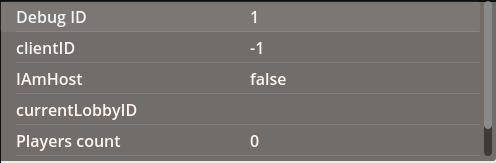
\includegraphics[width=0.5\textwidth]{resources/images/var-tree-preview.png}
    \caption{VarTree debug panel showing GDSync runtime variables: Debug ID, clientID, IAmHost flag, currentLobbyID, and Players count}
    \label{fig:var-tree-preview}
\end{figure}

This live inspection was particularly valuable during multiplayer debugging sessions where breakpoints were impractical due to timing-sensitive synchronization paths.

%-----------------------------------------------------------------------
\section{Summary}
\label{sec:implementation-summary}

This chapter presented the core implementation mechanisms of the HPC Sorting Serious Game:
\begin{itemize}
    \item \textbf{Card management} (705~lines in \texttt{card\_manager.gd}): generation, layout, sorting validation, and buffer contiguity checking.
    \item \textbf{Multiplayer extension} (1143~lines in \texttt{multiplayer\_card\_manager.gd}): host/client branching, \texttt{CardState} serialization protocol, GDSync function exposure, and state broadcast/reconciliation.
    \item \textbf{Barrier synchronization} (113~lines in \texttt{barrier\_manager.gd}): three-state machine implementing \texttt{\#pragma omp barrier} semantics with main-thread selection.
    \item \textbf{Web-export patch} (67~lines in \texttt{gdsync\_web\_patch.gd}): runtime LocalServer replacement preserving API contract.
    \item \textbf{Connection management} (348~lines in \texttt{connection\_manager.gd}): centralized GDSync signal wiring and typed player state.
    \item \textbf{Observability tooling}: structured logging and live variable inspection for multiplayer fault diagnosis.
\end{itemize}

\noindent The key repository entry points for readers who wish to inspect the full implementation:

\begin{table}[htbp]
    \centering
    \caption{Key source file locations}
    \begin{tabular}{@{}p{5cm}p{8.5cm}@{}}
        \toprule
        \textbf{Component}        & \textbf{Path}                                                             \\
        \midrule
        Card Manager (base)       & \texttt{scenes/CardScene/scripts/card\_manager.gd}                        \\
        Multiplayer Card Manager  & \texttt{scenes/Multiplayer/MultiplayerGame/multiplayer\_card\_manager.gd} \\
        Barrier Manager           & \texttt{scenes/Multiplayer/MultiplayerGame/barrier\_manager.gd}           \\
        Connection Manager        & \texttt{scenes/Multiplayer/connection\_manager.gd}                        \\
        Multiplayer Lobby         & \texttt{scenes/Multiplayer/Lobby/multiplayer\_lobby.gd}                   \\
        GDSync Web Patch          & \texttt{scenes/Multiplayer/GDSyncWebPatch/gdsync\_web\_patch.gd}          \\
        Signaling LocalServer     & \texttt{scenes/Multiplayer/GDSyncWebPatch/local\_server\_signaling.gd}    \\
        Signaling Client          & \texttt{scenes/Multiplayer/GDSyncWebPatch/signaling\_client.gd}           \\
        Scene Manager             & \texttt{scene\_manager.gd}                                                \\
        Signaling Server (Python) & \texttt{signaling-server/server.py}                                       \\
        \bottomrule
    \end{tabular}
\end{table}

\noindent Educational and operational effects of these mechanisms are interpreted in Chapter~\ref{ch:results}, while implementation failure modes and mitigations are documented in Chapter~\ref{ch:problems}.
